\section{RCPS Testbed Architecture}
\label{sec:Architecture}

Cyber-Physical Systems require design-time testing and analysis before deployment. Several CPS scenarios require strict safety certification due to the mission-critical nature of the operation, e.g. flight control and automation. It is often times impossible to test control algorithms, fault tolerance procedures etc. on the real system due to both cost and hardware accessibility issues. To counter these issues, there are two principle methods in which a CPS can be tested and analyzed: (1) Construct a complete model of the CPS in a simulation environment e.g. Simulink \cite{Simulink} and simulate the system while accounting for run-time scenarios, (2) Establish a testing environment that can closely resemble the real CPS in both hardware and software. The problem with simulations is that it is hard to establish the network topology, emulate the application network and base processing power while running a physics simulation  in the loop. Our RCPS architecture implements the latter alternative, as shown in Figure \ref{fig:architecture}. We propose a generic testing environment that uses embedded boards, programmable network switches and physics simulation machines to emulate real CPS deployments.

\begin{figure}[h]
	\centering
	\includegraphics[width=0.50\textwidth]{figs/architecture.png}
	\caption{Testbed Architecture}
	\label{fig:architecture}
\end{figure}

The testbed consists of 32 \emph{RCPS nodes}, each of which is a Beaglebone Black (BBB) \cite{BBB} development board running Linux. We execute a full software stack including a middleware and a component model, although much of this stack is not within the scope of this paper. For the subset of CPS we are interested in, the behavior of the CPS can be much more precisely emulated with these boards compared to running the applications inside of a standalone simulation. For example NASA's CubeSat Launch Initiative (CSLI) \cite{CubeSat} provides opportunities for nanosatellites to be deployed into space for research. CubeSats are small (4-inch long) satellites running low-power embedded boards and being prepared for interplanetary missions \cite{CubeSat_Mars} to Mars. A distributed set of CubeSats can be easily tested with this architecture if it can be integrated with a high-fidelity space flight simulator.  

The Gigabit Ethernet port of each BBB is connected to a \emph{Communication Network} switch. This is a programmable OpenFlow \cite{openflow} switch, allowing users to program the flowtable of the switch to control the routes that packets follow and completely configure the full network and subnets required for their emulated deployment.  Furthermore, the configurability of the communications network enables per-link or per-flow bandwidth throttling, enabling precise network emulation.  The primary \emph{Development and Control} machine, running our software development tools, communicates with the BBBs using this network. After software applications are deployed on this testbed, the characteristics of the real CPS network can be enforced on the application network traffic. Therefore, this network emulates the physical network which a distributed CPS would experience on deployment.

Each RCPS node is also connected to a \emph{Physics Network} using a 10/100 USB-to-Ethernet adapter, since the BBBs only have one gigabit ethernet port. This network is connected to a \emph{Physics Simulation Machine} running Cyber-Physical Systems simulations. Two such simulators are discussed in Section \ref{sec:Experiments}. This network provides the infrastructure necessary to emulate CPS sensing and actuation in the loop, allowing application software to periodically receive sensor data and open interfaces to output actuator commands to the simulation.

The Physics Simulation Machine closes the interaction loop for the testbed nodes, allowing the physical dynamics of the RCPS nodes to be simulated in the environment in which it would be deployed, \emph{e.g.} satellites' orbital mechanics and interactions can be simulated for a satellite cluster in low Earth orbit (LEO). 

%The physics simulation closes the loop for the testbed, allowing the physical dynamics of the testbed's hardware to be simulated in the environment in which it would be deployed.  Furthermore, an API allows the aspects of the simulation such as sensor data and control commands to be transmitted between the testbed and the simulation.

%One such simulator which supports this type of interface and has proven useful for the development and testing of CPS applications is Orbiter Space Flight Simulator.  Orbiter allows for very accurate gravitational dynamics simulation for systems in the solar system.  Using the API provided by the Orbiter add-on OrbConnect, programs can communicate with and control the spacecraft in the simulation.  

%Another more recent alternative to Orbiter, Kerbal Space Program (KSP), supports a wider range of physical system simulations, and expedites the process of simulation development and deployment.  Because KSP supports not only gravitational dynamics simulation, but also aerodynamic, rigid-body, and fluid simulation, it can be used to simulation systems which interact with these different domains.  Using the API provided by the KSP add-on KRPC (KSP remote procedure call), programs can control the state of the simulation and communicate with the systems in the simulation.  Whereas simulation development with orbiter required either the use of pre-existing models (e.g. the space-shuttle), or complete 3d modeling and specification of the system components to be simulated, simulation development with KSP is facilitated by the built-in tools KSP has to build aerospace/ground systems from their constituent components.  Because KSP has a large library of built-in components which have been modeled and can be composed together however the designer chooses, the capability to develop new simulations is greatly improved.  
\section{Design and Construction}
\label{sec:Construction}

The RCPS testbed was designed and constructed to be as self-contained as possible, while allowing for extensibility and modularity. The 32 BBB development boards were arranged on 4 laser-cut acrylic plates, with 8 boards on each plate, as shown in Figure \ref{fig:boards}. Holes on each plate route network and power supply cables from/to each board. With the communication network switch on top of these boards and the physics network switch on the bottom, the ensemble takes a total of 8U (rack units) of space. The primary power supply is an off-the-shelf 300 W power supply with custom cabling to fan-out power to all 32 boards in an efficient manner.  By configuring the testbed in this self-contained way, we can easily maintain it, monitor it, and move it should the need arise.  

\begin{figure}[h]
	\centering
	\includegraphics[width=0.40\textwidth]{figs/bbb.jpg}
	\caption{Beaglebone Black Boards - Custom Mounting}
	\label{fig:boards}
\end{figure}

Using a 13U server cabinet and standard mounting equipment, the network switches and simulation machines are mounted on either side of the development boards. Figure \ref{fig:testbed} shows the fully mounted testbed. The cabinet supports mountable base wheels which makes this setup easily portable. 

\begin{figure}[h]
	\centering
	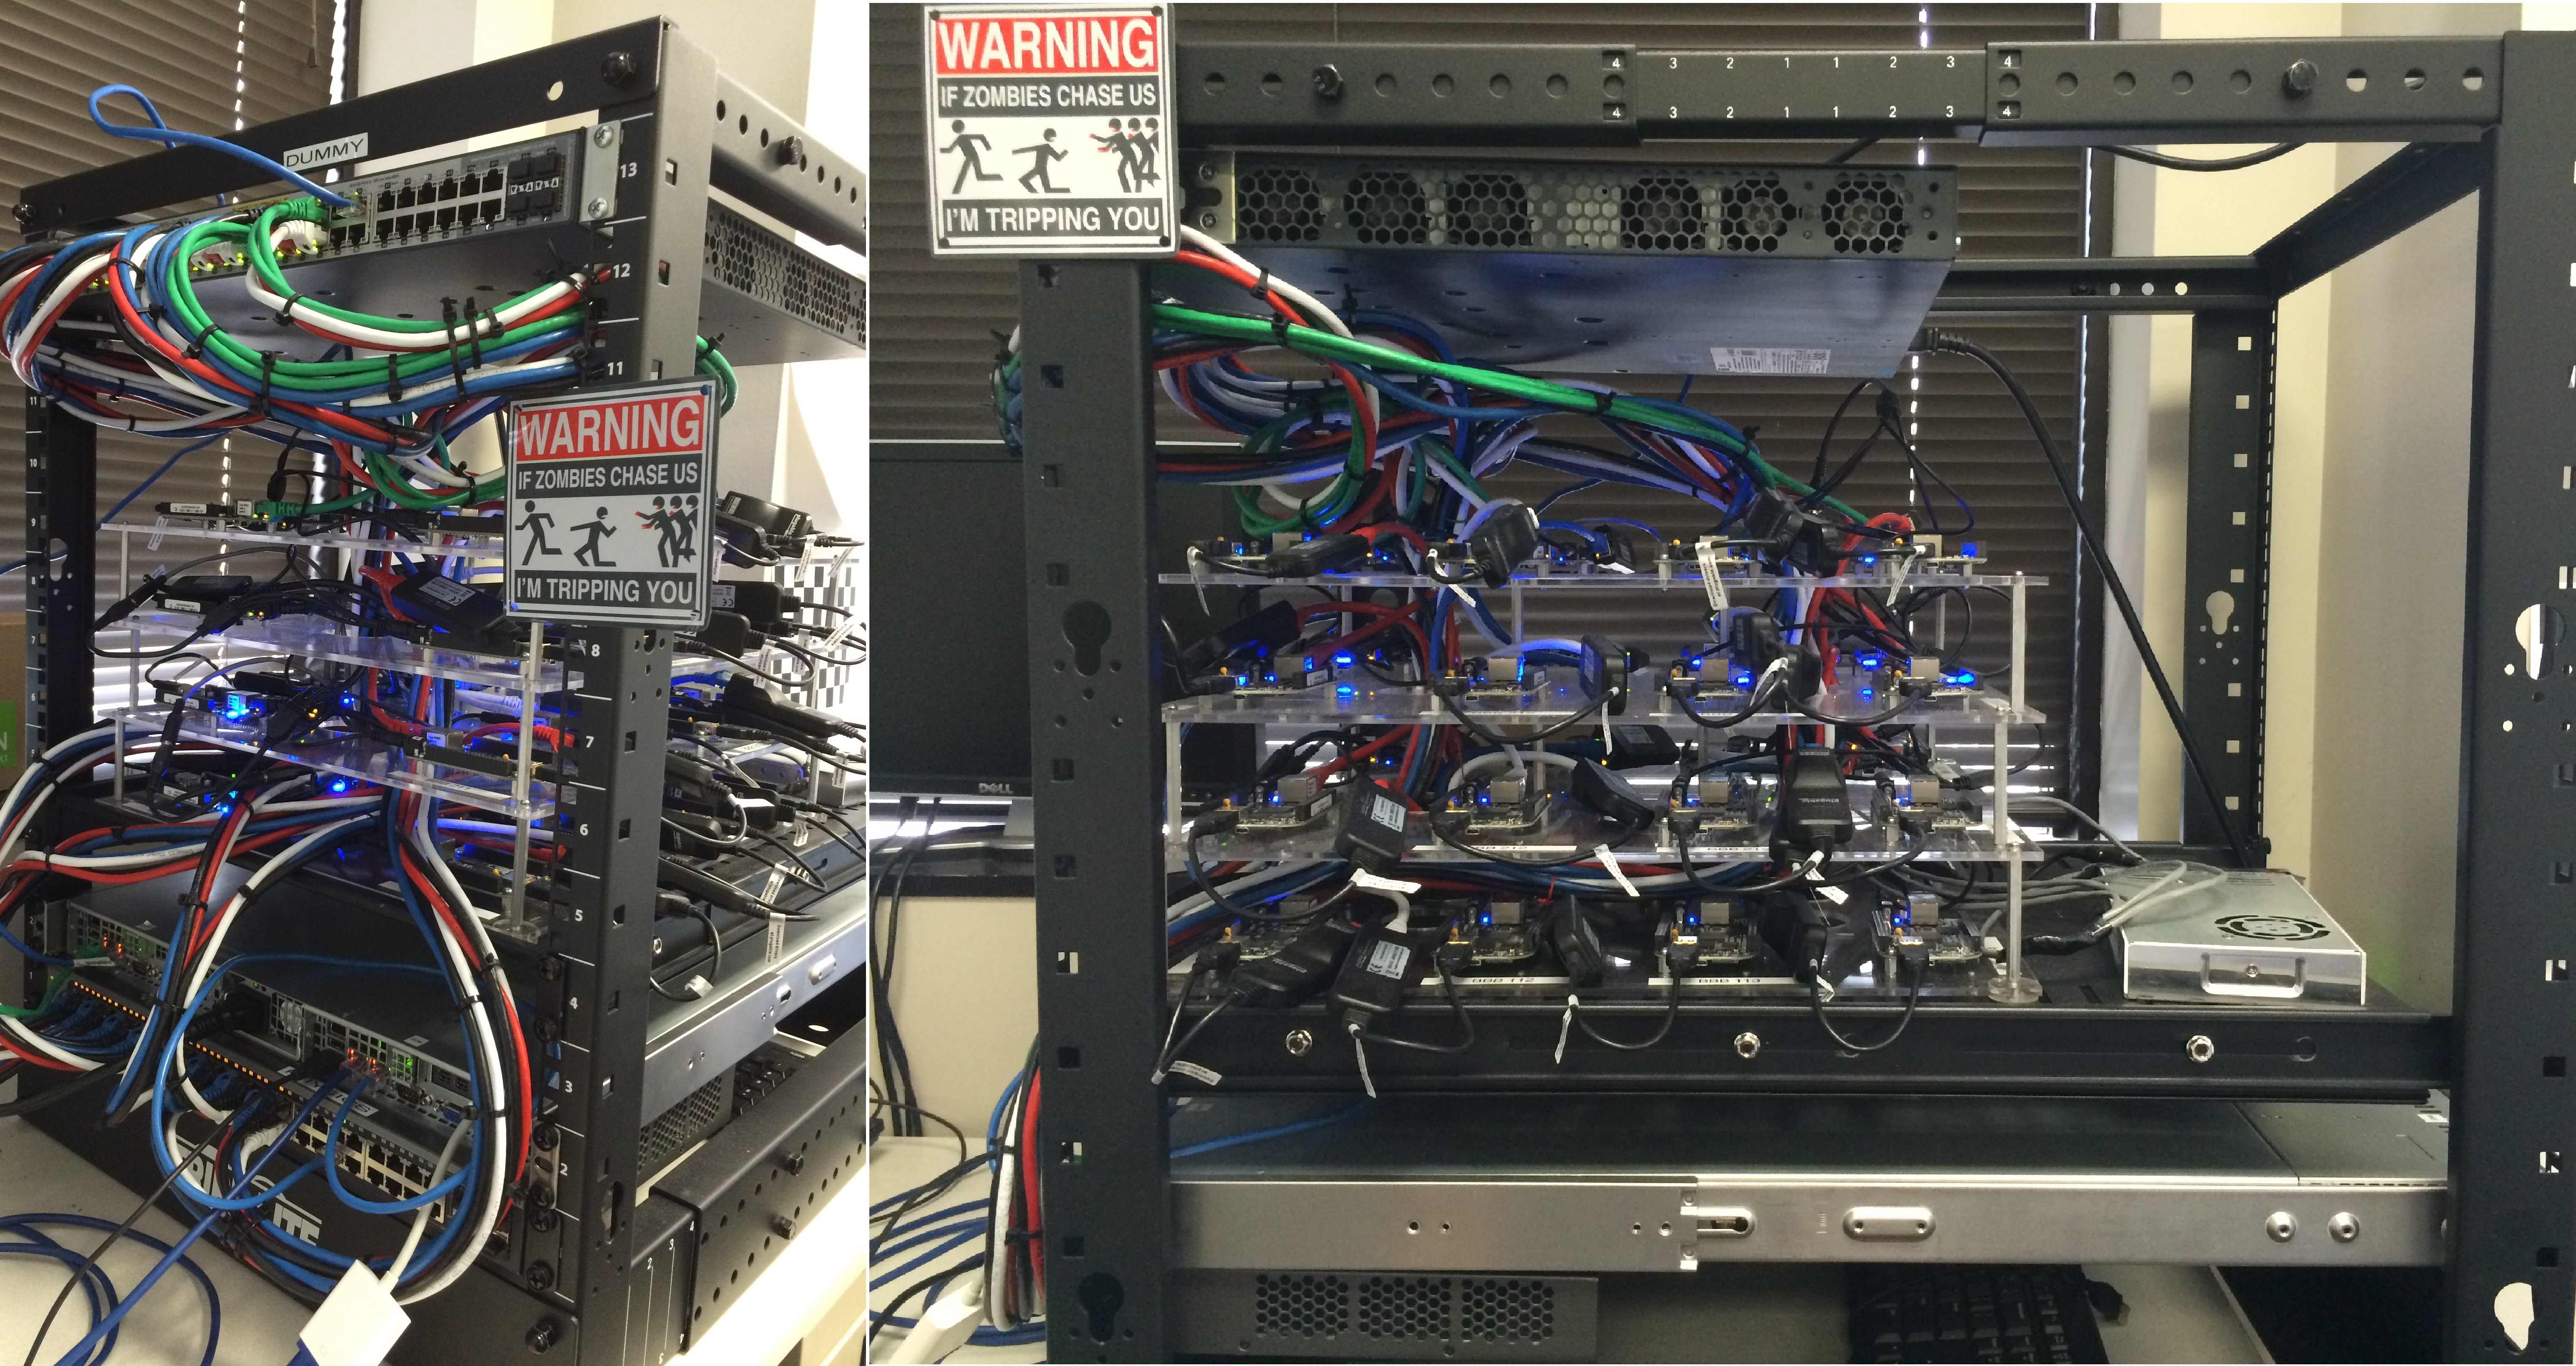
\includegraphics[width=0.50\textwidth]{figs/testbed.jpg}
	\caption{Constructed Testbed}
	\label{fig:testbed}
\end{figure}

\section{Experiments}
\label{sec:Experiments}

To validate our claims about the testbed, we have run several experiments that exercise its various aspects, primary of which is its utility in sensing, actuation and control of dynamic CPS scenarios. Our testing and experimentation parameters are as follows: (1) We use the Robot Operating System (ROS) \cite{ROS} middleware and follow component-based software development principles, (2) the physics simulation machine is running an appropriate high-fidelity simulation with exposed interfaces for input and output, (3) the development machine has full network access to all RCPS nodes in order to successfully develop, build and deploy applications on this distributed setup, (4) the applications have direct access to the physics simulation sensors emulating the real-world case where the sensor is part of the very board running the application, and lastly (5) the processes are able to log real-time activity to aid the monitoring infrastructure. This monitoring not only validates the behavior but also provides important measures such as operational time stamps that enable post-deployment timing analysis to assess the overall system performance.

This section briefly describes two unique scenarios pertaining to flight control dynamics. These are mission-critical CPS environments using different kinds of sensors, actuators and physics simulations. The real-time requirements of both set of applications are different and the average processing power capabilities of both systems can be approximated to our testbed nodes. Below, we categorize these experiments based on the physics simulators used.

\subsection{Orbiter Space Flight Simulator}

This is a scenario we have used in the past \cite{RSP-2014} to simulate a cluster of satellites. In our previous work, we used a minimal testbed to study mobile cloud infrastructure and integrated the Orbiter Space Flight Simulator \cite{Orbiter} to analyze a 3-Sat scenario. Now, with our RCPS testbed, the same scenario can be extended up to 32 satellites. Given the flexibility of this testbed, we can easily change the scenario to a 16-Sat cluster with 2 embedded boards per satellite or any similar variations. The amount of process concurrency and actuation is dependent primarily on the deployment infrastructure used. If a new test simply requires a new deployment model and some artifact XML files, then the testing mechanisms can be easily automated. 

\begin{figure}[h]
	\centering
	\includegraphics[width=0.45\textwidth]{figs/orbiter-1.png}
	\caption{32-Sat Scenario}
	\label{fig:orbiter}
\end{figure} 

This scenario, shown in Figure \ref{fig:orbiter}, consists of 32 small satellites orbiting as a satellite cluster in LEO.  The satellites each have different capabilities, with image sensors and imaging processors distributed throughout the cluster.  Each satellite runs a satellite flight control application which determines the state of the satellite, distributes the state to the rest of the cluster, tracks the states of the other satellites, and controls the satellite's thrusters.  This application communicates with a single orbit maintenance application in the cluster which maintains the orbital trajectories of all satellites in the cluster and instructs the cluster to perform maneuvers when needed.  In addition to these to applications, the cluster's resources are provided to applications which perform image sensing, image processing, and communication tasks.  

\begin{figure}[h]
	\centering
	\includegraphics[width=0.45\textwidth]{figs/orbiter-2.png}
	\caption{Scatter Maneuver}
	\label{fig:orbiter_2}
\end{figure}

It must be noted in this scenario that Orbiter executes only in Windows. The Physics simulation machine is a dual-boot setup capable of supporting a wide range of simulation due to both its CPU power (16 cores with 16 GB of RAM) and its NVIDIA Quadro K1200 graphics card. Another limitation to Orbiter is that the interface used to communicate with Orbiter, OrbConnect, does not provide the full range of attitude control for the satellites, although Orbiter supports this level of actuation. Therefore, even though the scenario exercises a scatter maneuver on receiving a critical command from the ground station, as shown in Figure \ref{fig:orbiter_2}, the behavior of this CPS is slightly inconsistent with the real-world scenario. Due to this, we have moved to a different flight simulator, as described below.  

One of the relevant and interesting aspects of this satellite example is the networking required between the satellites.  Because of the nature of the orbital mechanics governing the motion of the satellites, the distances between each of the satellites in the cluster varies periodically over time as a sinusoidal function.  This deterministic variation in distance directly correlates to a deterministic network capacity variation which also is periodic according to the orbital period of the cluster.  Because this information can be easily retrieved from the simulation, it can be used to alter the emulated network characteristics.  Since the variation is deterministic and calculable, the emulated network characteristics can be measured and compared against the calculated, predicted network characteristics. 

\subsection{Kerbal Space Program}

Kerbal Space Program \cite{KSP} (KSP) is a widely popular space flight simulator for a variety of platforms including Linux, OS X and Windows. In this game, players get to manage a space program, designing and building spacecrafts and exploring celestial bodies. 

While KSP does not provide a perfect simulation of reality, it has been widely praised for its component-based design and development process coupled with aerodynamic, gravitational, and rigid-body interaction and simulation. In this simulation, every man-made object follows Newtonian dynamics. Rocket thrust and aerodynamic forces are accurately applied to the vehicles based on the directions and precise positions in which the force-affected elements are mounted on the vessel. Using KSP, we have modeled scenarios for a variety of flight missions including interplanetary travel. In this section, we briefly describe an aircraft flight controller that was designed and tested using the RCPS testbed and KSP.

This CPS scenario is a flight controller application used to completely control a KSP aircraft from the primary space-plane hanger to a destination airport. The application processes require inputs from KSP e.g. sensor data about pitch, roll, yaw, mean altitude etc. and interfaces to control the flight dynamics e.g. thrust, pitch and heading. If these interfaces are setup, then the processes can periodically retrieve flight telemetry and provide commands for course correction and feedback control.

\begin{figure}[h]
	\centering
	\includegraphics[width=0.50\textwidth]{figs/ksp.png}
	\caption{Stearwing A300 PID Control}
	\label{fig:ksp}
\end{figure} 

Using an open source project called kRPC \cite{kRPC} (Kerbal Remote Procedure Call Server), the BBB nodes running CPS processes are provided with an interface to the simulation. Figure \ref{fig:ksp} shows the Stearwing A300 aircraft taking off from the space-plane hanger and stabilizing at a cruising altitude of 2000 meters, as shown in Figure \ref{fig:krpc}. Each control unit in the aircraft is simulated by a BBB. It is critical to incorporate redundancy in all components and connections to assure that the system can survive runtime failures, especially in airborne software \cite{airborne_software} \cite{kornecki2004approaches}. So, many of the RCPS nodes in our testbed act as redundant sensors, all connected to KSP, receiving and periodically publishing messages. If one of the nodes in the testbed fails, either due to a hardware anomaly or a software fault, then the rest of the nodes are used to arrive at a general agreement regarding the sensor value to be considered for control. 

\begin{figure}[h]
	\centering
	\includegraphics[width=0.50\textwidth]{figs/krpc.jpg}
	\caption{Stearwing A300 Altitude Profile}
	\label{fig:krpc}
\end{figure} 

Like Orbiter, using KSP also has its limitations. However, many such limitations are characteristic of the simulation interface and not the simulation itself. The C++ interface library we have used does not provide for the means to control multiple \emph{vessels} in the simulation. Instead, developers are provided the complete control API for the \emph{active vessel}, which is the vessel currently in focus in the game. Although such an interface is currently in the works, as it stands, KSP is a good solution for testing CPS use cases where a set of embedded boards are coordinating and controlling a single vessel or medium. Also, the KSP community provides several crowd-made modifications to the base game that supports various vehicle parts, aerodynamic changes, and drag models that enable researchers to build and test a variety of systems including cars, rovers, UAV swarms, robots, and even laser-guided systems. The open nature of this simulator makes this a realistic testing environment for dynamic CPS specifications.   
 
%The scenario we developed for testing and simulation with KSP is an airplane guidance and control system which uses sensor data about the plane together with pre-selected waypoints to perform autopiloting of the plane from take-off to landing.


\section{Discussion}
\label{sec:Discussion}

Despite the capabilities of this RCPS testbed architecture in analyzing distributed resilient CPS, its limitations must be evaluated with respect to system applicability and experimental validity. Such limitations govern the types of CPS which can be developed and tested with this architecture, as well as the scale of the systems to which this architecture can be used. 

Because much of the testbed infrastructure is networking, and because much of the distributed application development and testing comes from the network infrastructure provided by the CPS (and therefore emulated by the testbed), one of the most critical aspects of the CPS testbed to analyze is the networking infrastructure.  In this testbed's architecture, there are distinct networks reserved for application level network traffic, i.e. data which would flow on a real network in the deployed system, and for physics simulation network traffic, i.e. data which would be relayed by hardware directly connected to the embedded boards.  The simulation network traffic allows the embedded hosts in the network to retrieve sensor data and send actuator commands to simulated hardware on the physics simulation node.  Because this network is one of the major differences between the testbed and the real system, it must be carefully analyzed to determine how accurately it behaves with respect to the real system.  

The actual network in the testbed is comprised of two parts: (1) a Gigabit network switch which is dedicated to the physics simulation traffic, and (2) the 10/100 USB-Ethernet adapters on each board which allow a direct connection to the physics network.  The USB-Ethernet adapters on the boards do not allow the boards to utilize the full capabilities of their Ethernet connections to the physics network, but provide sufficient bandwidth for many sensor applications. For a single host, many sensor streams or a few high-data-rate sensors can adversely affect the host's sensor timing and services, thus affecting the system overall. High-resolution or high-rate image-based sensing on a certain host may degrade the performance of the host's physics network link, but should not affect the rest of the physics network. However, many such high-bandwidth sensing applications distributed across the cluster may degrade the overall performance of the physics network.  Because in the real system, these high bandwidth data streams would be completely isolated and independent, this type of network performance degradation can cause the testbed applications' behavior to deviate from the real system applications' behavior.  

The other network which plays an critical role in the testbed is the application network, which handles all network traffic for the system which would actually be transmitted on a network in the deployed system.  The purpose of this network is to enforce on the applications' network traffic the same network characteristics as would be seen in the real system.  Because the wired testbed application network is managed by a smart network switch using OpenFlow, many different and concurrent topologies can be enforced, and every link in the networks can be configured with different, varying bandwidth.  For many types of networks, this type of network emulation is sufficiently accurate and will provide meaningful, useful test results.  However, certain types of networks in deployed systems cannot be easily emulated with this setup, for instance, wireless networks with high error rates and high packet-loss or collision rates are difficult to emulate using this network infrastructure.  Moreover, the environmental effects such as multi-path or obstruction may be difficult or impossible to emulate.  
%can't do all integration testing
%usb-ethernet -> limitation for physics possibly -> what scenarios
%switches can be limitations depending on applications and such -> to what can they support?
%processing limitations -> dependent on testbed -> hardware prototyping boards should be used for relevant hardware
%how does the system/testbed scale: switches? openflow?

\section{Future Work/Extensions}
\label{sec:Extensions}
\subsection{Experiments}
With this testbed, we are able to analyze different systems and multiple different aspects of those systems.  Our primary goal with this testbed is the general analysis of distributed CPS through certain aspects such as resiliency and security.  Based on this goal, we will analyze how certain systems behave with respect to fault tolerance, fault propagation, failure mitigation, and reconfiguration.  These experiments govern some aspects of the resilience of the systems, and we will specifically focus on systems such as the aircraft software example mentioned above, as well as UAV swarms, autonomous cars, and traffic grid control systems.  

Another critical aspect of these distributed CPS which we wish to analyze is their security.  Because our testbed encompasses the physics, the hardware, the software, and the network of the CPS, we can analyze multiple attack vectors and their impact on the applications and the software infrastructure.  These experiments can be coupled with the resilience experiments mentioned above to analyze the capability of attackers to achieve specific goals of bringing down certain subsystems or the overall system.  
\subsection{Testbed Analysis}
To better understand the capabilities and limitations of the testbed, we will measure such testbed characteristics as: (1) the effect the USB/Ethernet adapter has on communications delay, timing, and jitter, (2) the effect OpenFlow link management has on applications' usable bandwidth, and (3) the effect OpenFlow dynamically altering flows and bandwidth re-allocation has on active traffic.
\subsection{System Analysis}
Using our deployment and management tool suite, we can analyze CPS deployments for system-level properties such as (1) Buffer Space Requirements satisfaction and per-link network traffic delay, (2) timing and schedulability satisfaction without deadline violations or system-wide deadlocks.
\subsubsection{Network Analysis}
Because we can accurately and precisely emulate the CPS network characteristics on the testbed, we can analyze the performance of the networked applications by measuring their utilized buffer space and their communication delay.  These measurements, performed automatically throughout the system, provide a clearer insight into the network services provided by the system and the resource utilization required by the applications on the system.  Comparing these requirements and services we can analyze the performance of the applications to determine the affect the network and its service capacity has on the applications' behaviors.  
\subsubsection{Timing Analysis}
Timing analysis of models of CPS are useful only when the modeling abstractions for the CPS domain are uncompromising and the analysis techniques can be validated by testing in an approximated CPS testbed. This is one of our primary goals with the RCPS testbed. In previous work, we have shown our timing analysis methods \cite{MoDeVVa} \cite{SEUS} for component-based distributed CPS. Using a generic \emph{I/O component} for integration with physics simulation, we are working on modeling and analyzing the temporal behavior of software components while interacting with simulations. Our monitoring framework used with this testbed provides a strong infrastructure and the necessary inputs for timing verification.